We now investigate whether word orders as found in natural language reflect optimization for the memory--surprisal trade-off more generally.
To this end, we compare the memory--surprisal trade-offs of 52 actual languages to those of counterfactual baseline languages, which differ from the actual languages only in their word order rules. This method of comparison against counterfactual baseline languages was introduced by \citet{gildea-optimizing-2007,gildea-grammars-2010} has been applied to study optimization-based models of word order universals by \citet{futrell-large-scale-2015}, \citet{gildea-human-2015}, and \citet{hahn2020universals}.

Here, we describe how we measure the memory--surprisal trade-off in corpora, and how we generate counterfactual baseline languages. In Section~\ref{sec:main-experiment-results}, we compare the trade-off in real corpora against the trade-off in the counterfactual baselines.

\subsection{Measuring the memory--surprisal trade-off in corpora}

The key to evaluating the memory-surprisal tradeoff from corpus data is the set of quantities $I_t$, the  mutual information between words at distance $t$ conditional on the intervening words. 
All that is required is to estimate the quantities $I_t$; then these can be plugged in to Theorem~\ref{prop:suboptimal} to give a lower bound on the memory--surprisal trade-off. 

The quantities $I_t$ can be estimated as the difference between the average surprisal of Markov models that have access to the last $t-1$ or $t$ words.
That is, if we have a $t$th-order Markov model with average surprisal
\begin{equation*}
    S_t = H[w_t | w_0, \dots, w_{t-1}]
\end{equation*}
and a $(t-1)$th-order Markov model with average surprisal
\begin{equation*}
    S_{t-1} = H[w_t | w_1, \dots, w_{t-1}],
\end{equation*}
then we can calculate $I_t$ straightforwardly in the following way:
\begin{align}
    \nonumber
    I_t &= I[w_t : w_0 | w_1, \dots, w_{t-1}] \\
    \nonumber
    &= S_{t-1} - S_t.
\end{align}
Therefore, to evaluate $I_t$, all we need is a way of fitting Markov models of order $t$ and $t-1$. Then the average surprisal values can be extracted from these models straightforwardly.

To fit Markov models to the data, we use neural language models. In particular, we use Recurrent Neural Networks with Long Short-Term Memory architectures \citep{hochreiter-long-1997}. 
Neural network models are the basis of the state-of-the art in statistical modeling of language and in predicting the surprisal effect on reading times~\citep{frank-insensitivity-2011,goodkind-predictive-2018}.
See Supplementary Materials Section X for details on how these models were fit to data, and see Supplementary Materials Sections Y and Z for control studies using other methods of estimating $I_t$ (based on $n$-gram models and PCFG chart parsers). The results of these control studies are in agreement with the neural network results presented in this section.

In order to evaluate the values $S_t$, we calculated the average surprisal under the $t$th-order Markov model on held-out data, different from the data that was used to train the model. By evaluating on held-out data, we avoid underestimating the value of $S_t$ due to overfitting.

\subsection{Data}
We draw on corpora annotated with syntactic structures.
The Universal Dependencies project has compiled such annotated corpora for several dozen languages~\citep{nivre-universal-2017}.
These are annotated in the format of Dependency Grammar.

\paragraph{Dependency Grammar}
In dependency corpora, sentences are annotated with \emph{dependency trees} (Figure~\ref{fig:dependency}).
These are directed trees describing the grammatical relations among words. For example, the arcs labeled ``obj'' represent that the noun in question is the \emph{direct object} if the verb, rather than e.g. the subject or an indirect object.
A dependency arc is drawn from a \emph{head} (e.g. TODO in Figure TODO) to a \emph{dependent} (e.g. TODO).
Dependency trees can be defined in terms of many different syntactic theories \citep{corbett1993heads}.
Although there are some differences in how different formalisms would draw trees for certain sentences, there is broad enough agreement about dependency trees that it has been possible to develop large-scale dependency-annotated corpora of text from dozens of languages \cite{nivre2017universal}.

\begin{figure}
\centering
\begin{dependency}[theme = simple]
   \begin{deptext}[column sep=1em]
	   I \&	   wrote \& risāla \& li \& sadīq  \\
   \end{deptext}
	%   \deproot{3}{ROOT}
   \depedge{1}{2}{obj}
	%   \depedge[edge start x offset=-6pt]{2}{5}{ATT}
   \depedge{1}{4}{obl}
   \depedge{4}{3}{case}
   %\depedge[arc angle=50]{7}{6}{ATT}
\end{dependency}
	\caption{TODO Dependencies example}\label{fig:dependency}
\end{figure}

\paragraph{Selection of Languages}
We considered all languages for which there are Universal Dependencies 2.4 treebanks with a total of at least 500 sentences of training data.
We excluded data from historical languages.\footnote{Historical languages excluded: Ancient Greek, Classical Chinese, Coptic, Gothic, Latin, Old Church Slavonic, Old French.}
%While running this experiment, data from additional languages became available that also had enough data, through the Universal Dependencies 2.4 release. 
This resulted in 54 languages.

\paragraph{Processing of Corpora}
For each of these languages, we pooled all available corpora in one dataset.
We excluded corpora that primarily contain code-switched text\footnote{Hindi English corpus}, or text created by non-native speakers.\footnote{ESL for English, CFL for Chinese.}
Most Universal Dependencies corpora have a predefined split into \emph{training}, \emph{held-out} (also known as \emph{development}), and \emph{test} partitions.
%While larger corpora have all three partitions, smaller corpora often have only some of these partitions.
In most cases, we used the predefined data split, separately pooling data from the different partitions. 
For some languages with little data, there is no predefined training partition, or the training partition is smaller than the other partitions.
In these cases, we redefined the split to obtain more training data.
For these languages, we pooled all the available partitions, used 100 randomly selected sentences as held-out data, and used the remainder as training data.\footnote{This affects Amharic, Armenian, Breton, Buryat, Cantonese, Faroese, Kazakh, Kurmanji, Naija, Thai, and Uyghur.}
We provide the sizes of the resulting datasets in Table~\ref{tab:corpora}.

\subsection{Defining baselines}

We construct counterfactual ordering grammars that define consistent ordering rules similar to those found in actual languages.
For instance, these grammars will specify which dependents precede or follow their heads (e.g., whether objects follow or precede verbs, whether adjectives follow or precede nouns), and the relative order of different dependents on the same side of the head (e.g., whether noun phrases have order adjective-numeral-noun or numeral-adjective-noun). Our formalism of ordering grammars adapts the method of \citet{gildea-optimizing-2007,gildea-grammars-2010,gildea-human-2015} to the setting of dependency corpora, following \citet{futrell-large-scale-2015} and \citet{hahn2020universals}.


\begin{figure}
\centering
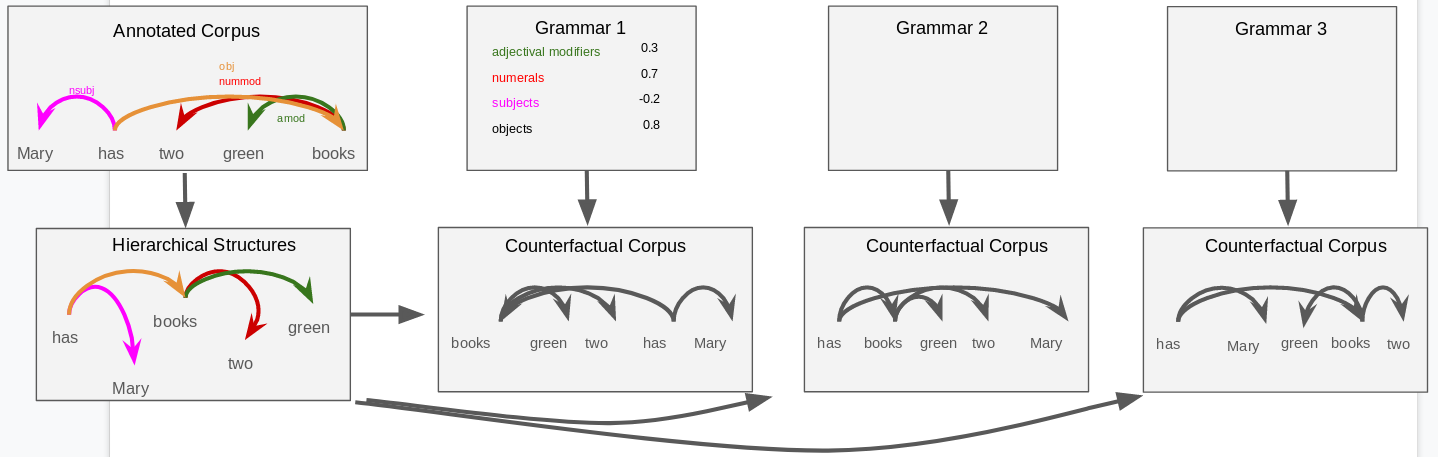
\includegraphics[width=\textwidth]{figures-gdrive/counterfactual-languages.png}
	\caption{\note{Can say more here to explain how it works} Estimating chance by constructing counterfactual grammars and languages.\jd{this figure is again blurry for me. also looks like there's sth in the background on the left?}}\label{fig:grammars}
\end{figure}


Universal Dependencies defines 37 universal syntactic relations that are used to label dependency arcs across all corpora.
These relations encode cross-linguistically meaningful relations such as subjects, objects, and adjectival modifiers.
We define ordering grammars by assigning a parameter $a_\tau \in [-1,1]$ to every one of these 37 universal syntactic relations.
Relations sometimes have language-specific subtypes; we do not distinguish these subtypes.

Following Gildea and colleagues, this parameter defines how dependents are ordered relative to their head:
Given a head and a set of dependents, we order each dependents by the parameter $a_\tau$ assigned to the syntactic relation linking it to the head.
Dependents with negative weights are placed to the left of the head; dependents with positive weights are placed to the right.

Ordering grammars describe languages that have consistent word order:
For instance, the subject is consistently ordered before or after the verb, depending on whether the parameter for the verb-subject dependency is positive or negative.

We construct baseline grammars by randomly sampling the parameters $a_\tau$.
Such baseline grammars define languages that have consistent word order, but do not exhibit preferences for specific word order patterns.


In actual languages, the ordering of words is largely determined by the syntactic relations (CITE).
However, certain kinds of rules cannot be modeled by our word order grammars, such as rules sensitive to the category of the dependent (e.g., differences between nominal and pronominal objects).
Word order freedom also is not modeled.
In this sense, ordering grammars represent approximations to the kinds of ordering rules found in natural language \citep{gildea-optimizing-2007, gildea-grammars-2010, gildea-human-2015}.
See Section (Discussion) for further discussion.


\subsection{Results}

\begin{figure}
	\begin{center}
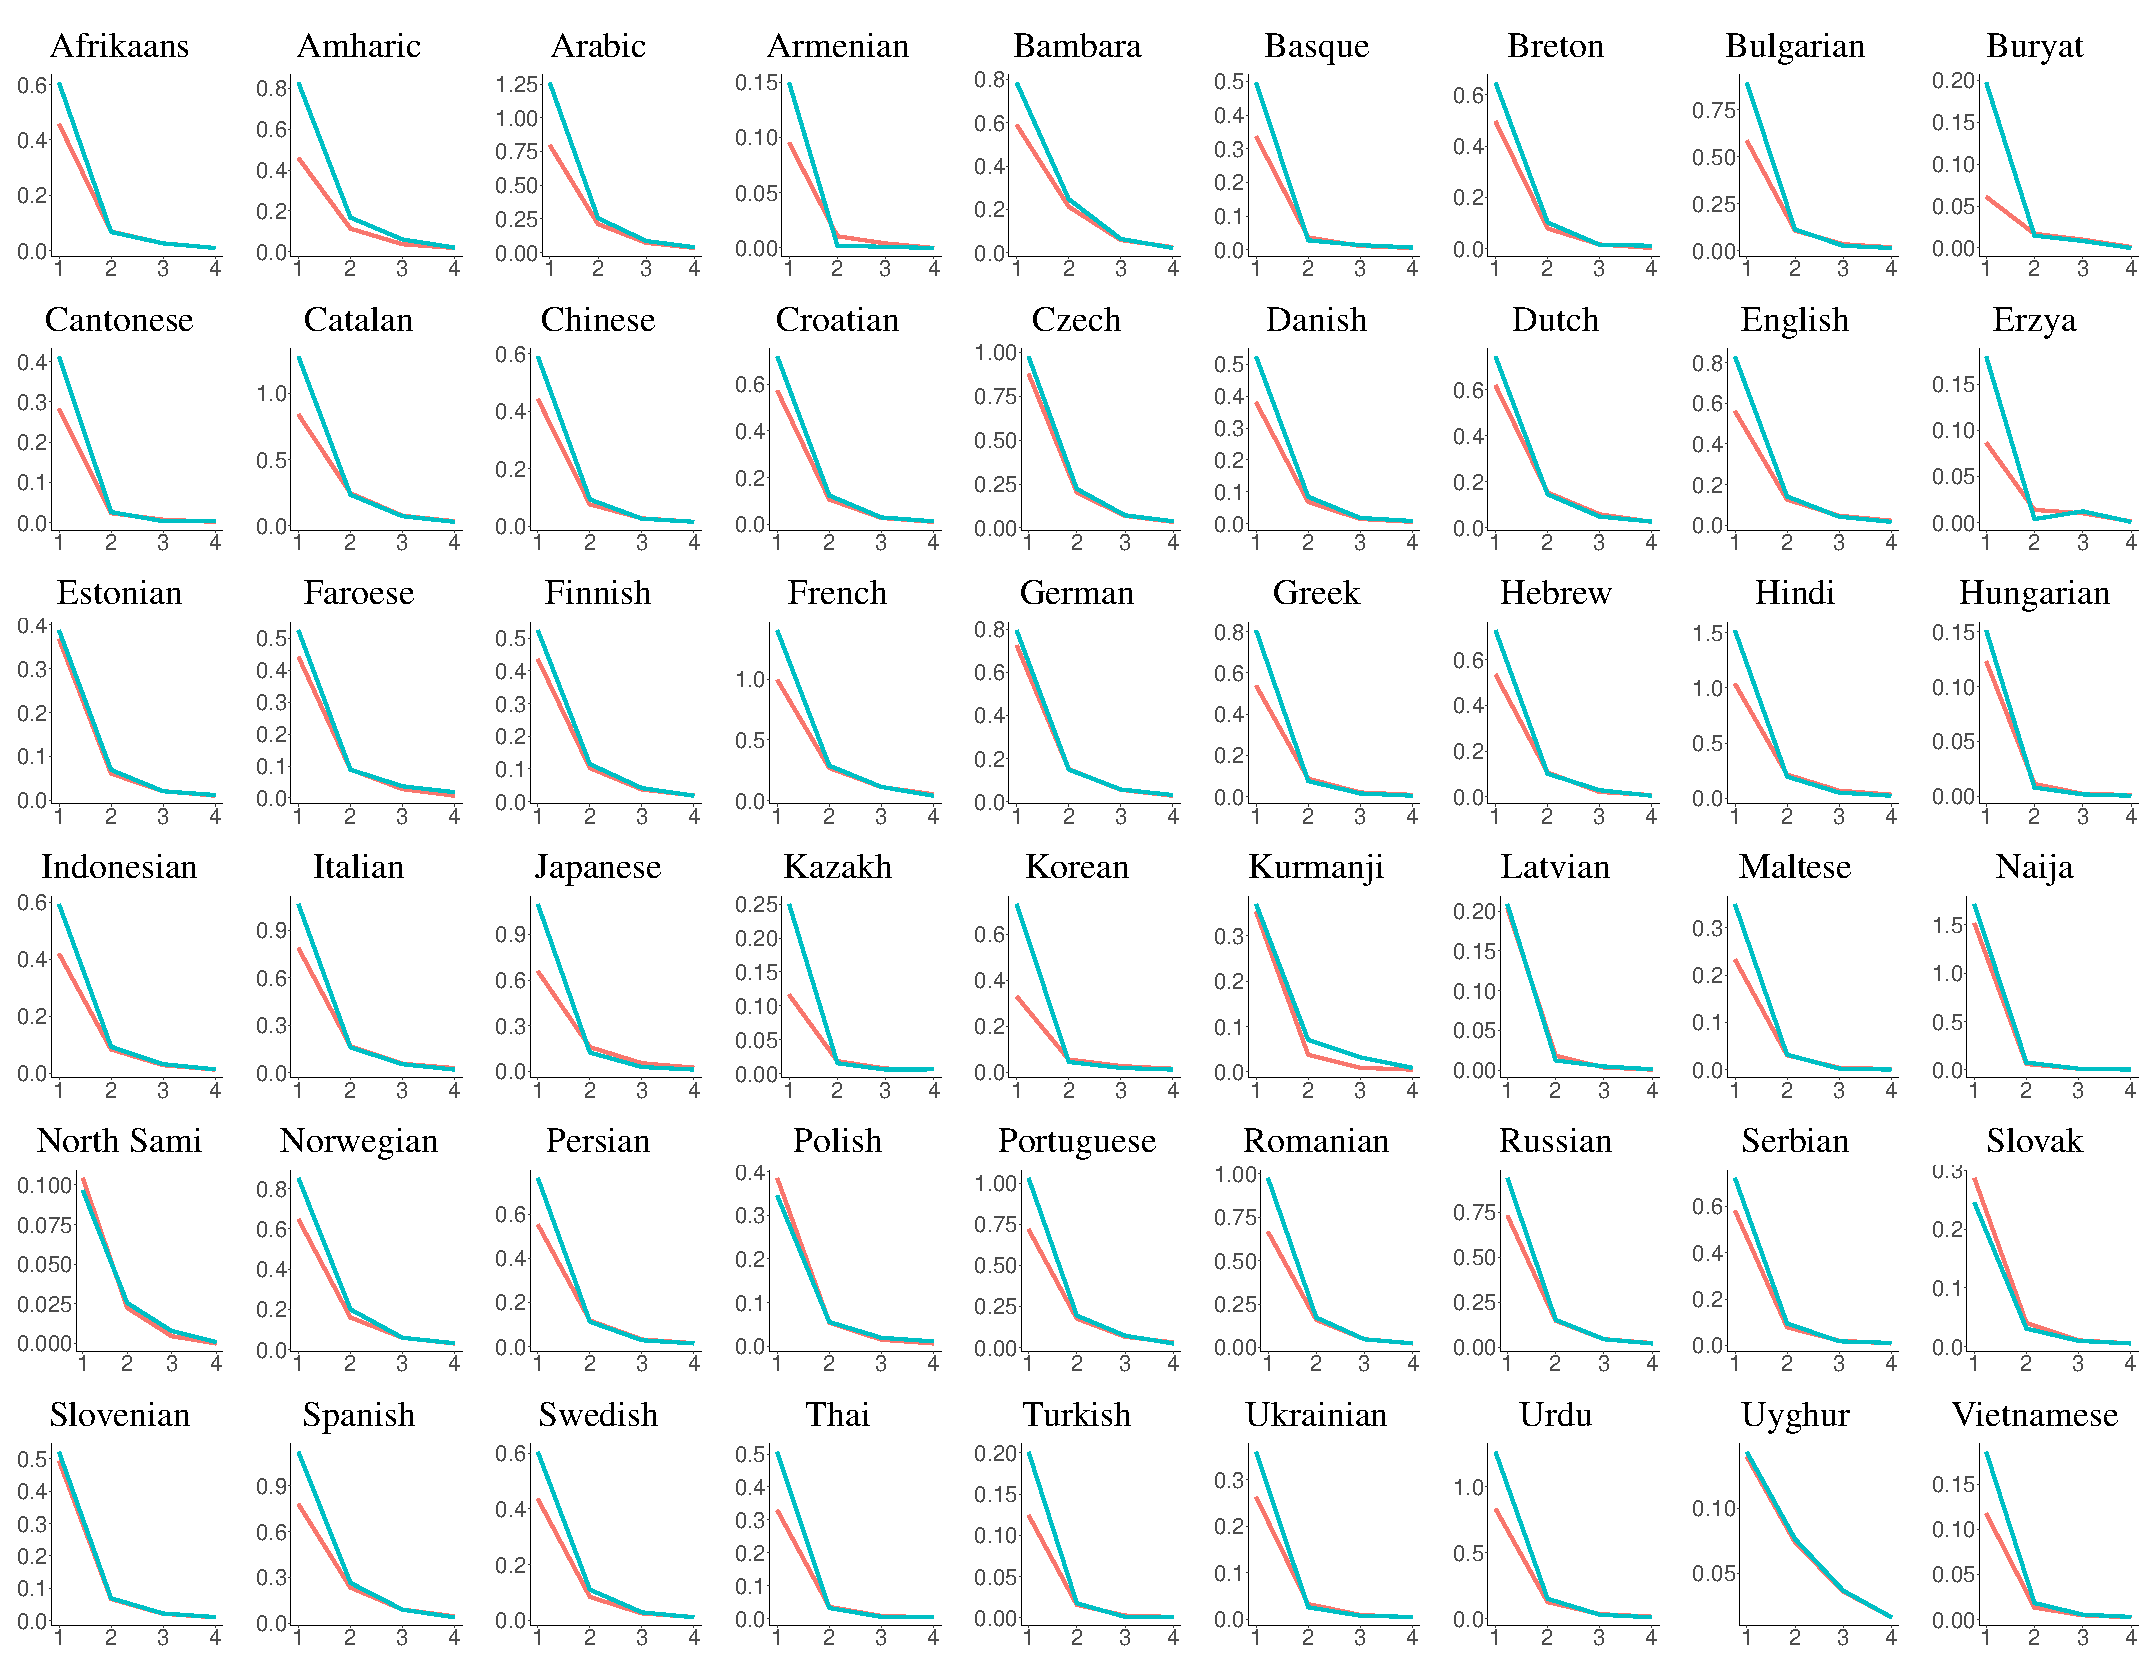
\includegraphics[width=\textwidth]{it-table.pdf}
\end{center}
	\caption{$I_t$ (y-axis) as a function of $t$ (x-axis), for real (blue) and counterfactual (red) orders. We plot the median over all runs of the neural network estimator, and over all random grammars.}\label{fig:it}
\end{figure}



\begin{figure}
	\begin{center}
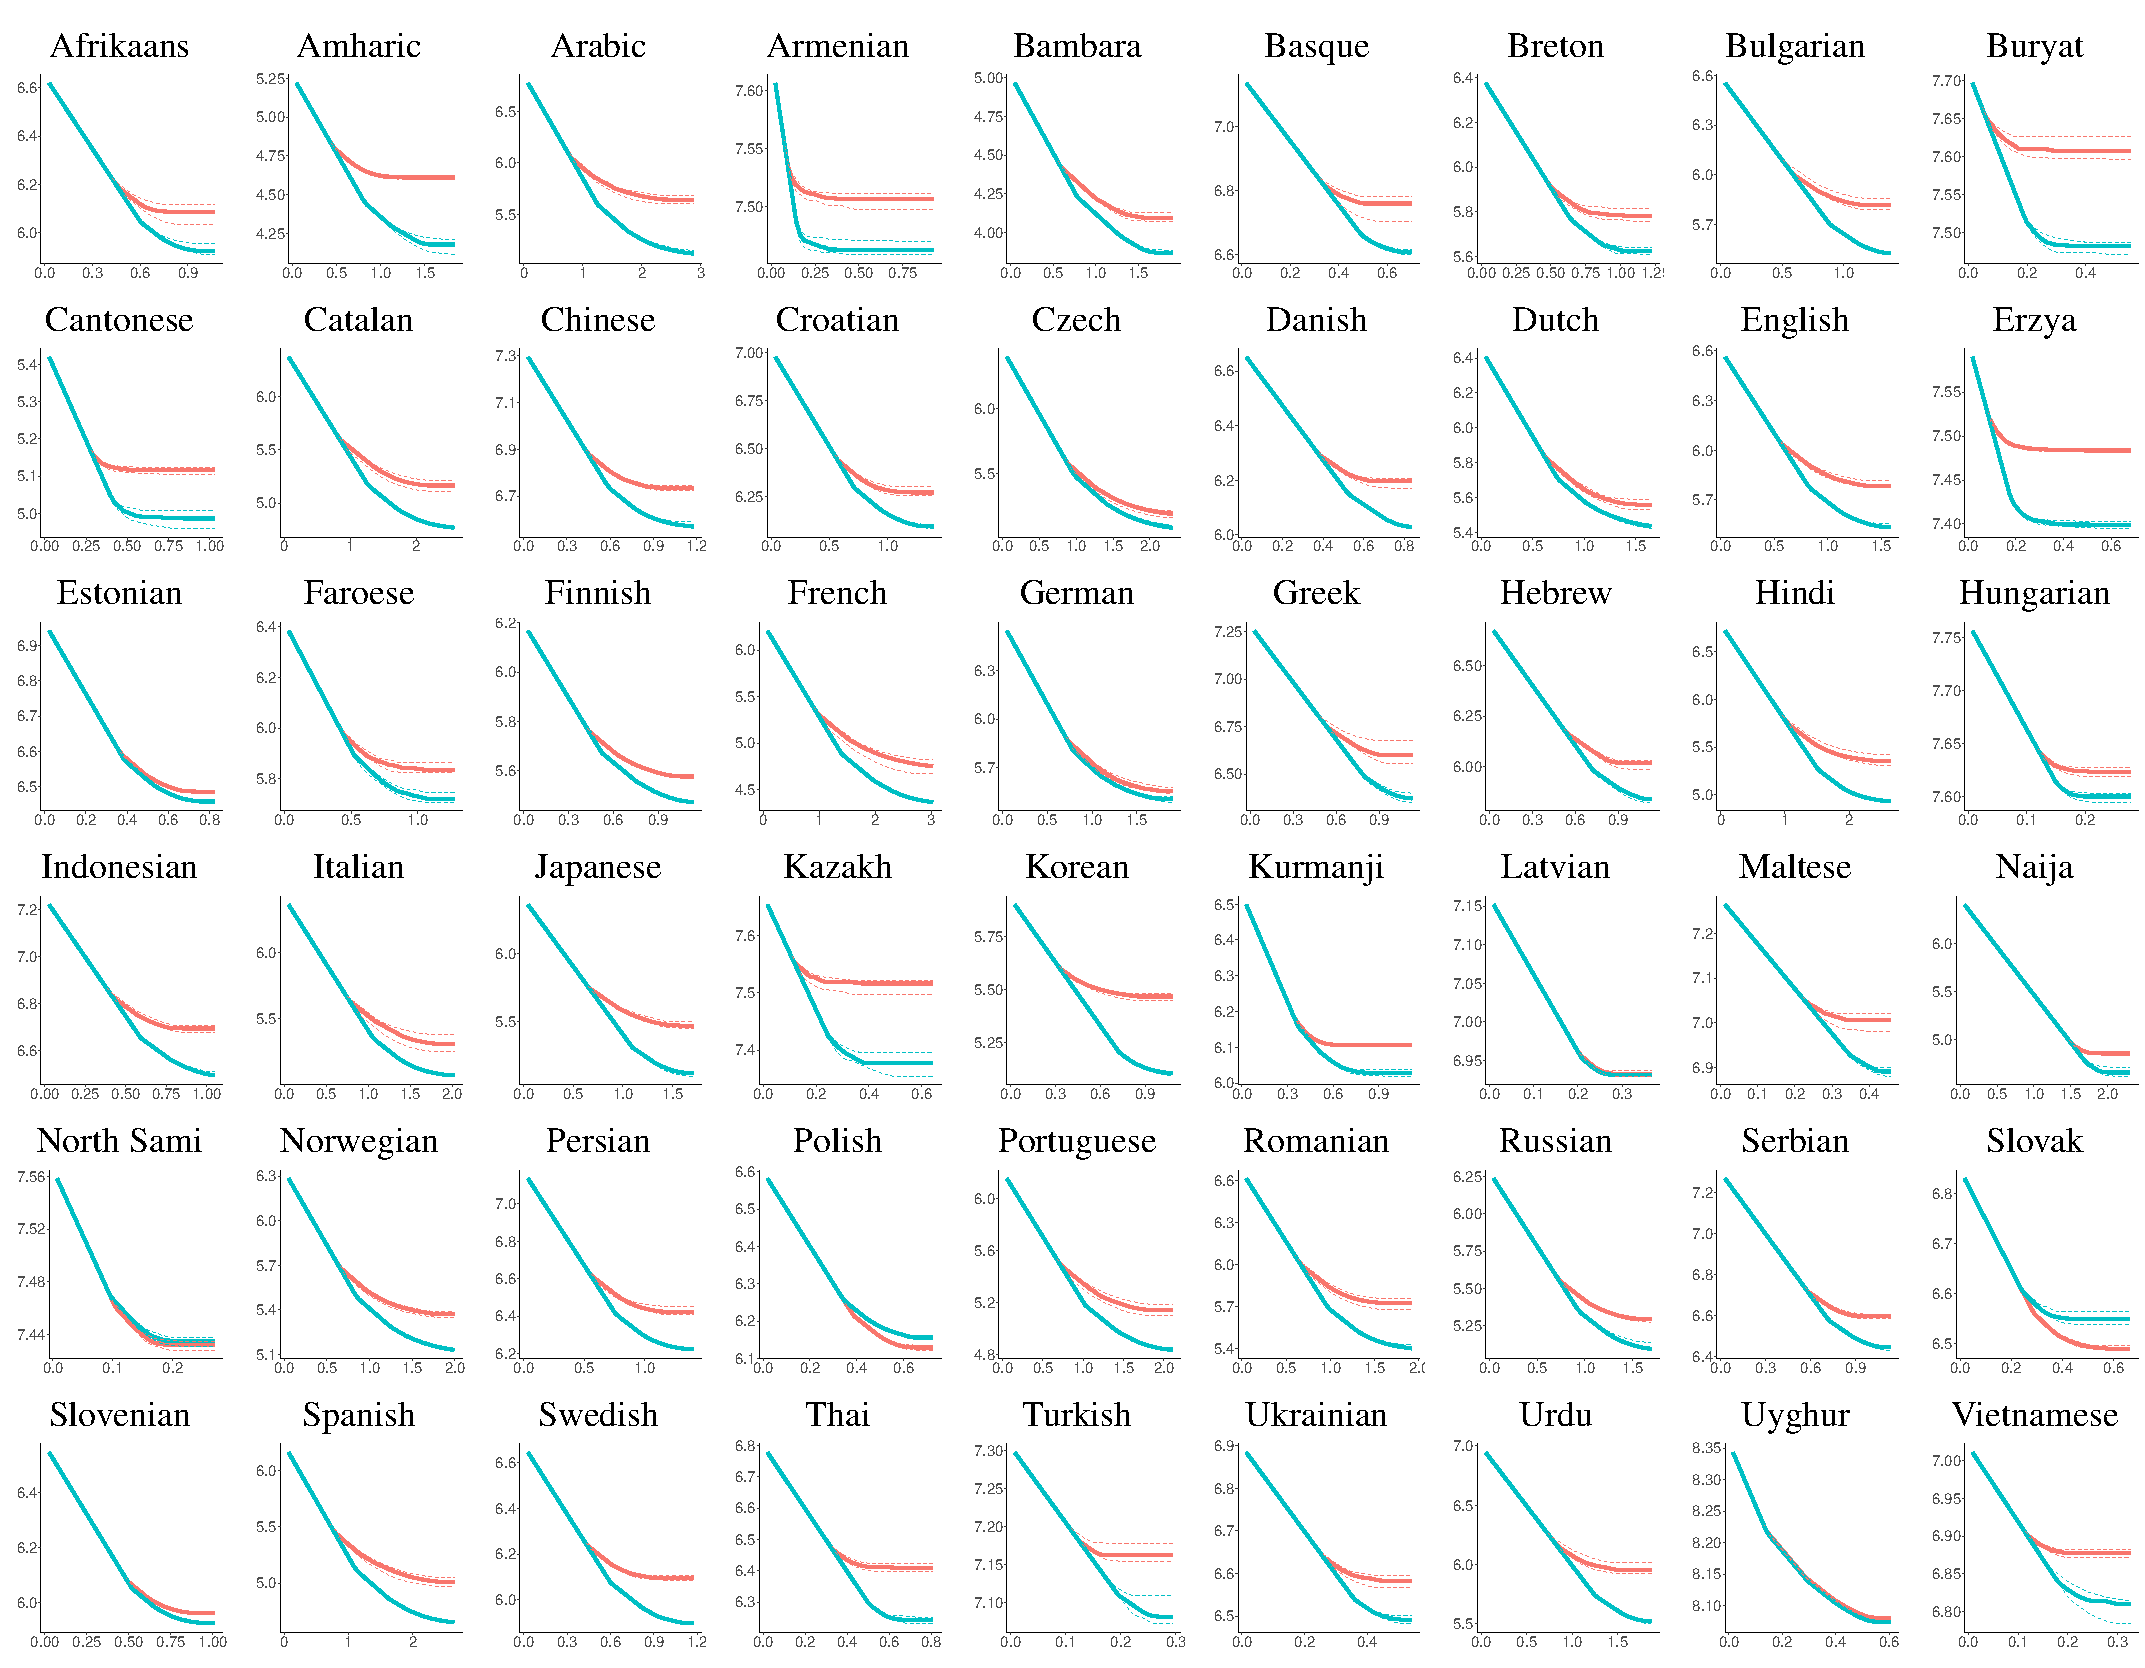
\includegraphics[width=\textwidth]{results-table.pdf}
\end{center}
	\caption{Median surprisal (y-axis) at given memory level (x-axis), for real orders (blue) and random baseline grammars (red). We provide 95\% confidence bands. These are computed over different runs of the estimation algorithm for the real orders, and over different runs \emph{and} different grammars for the baseline grammars.}\label{fig:median-table}
\end{figure}


\begin{figure}
	\begin{center}
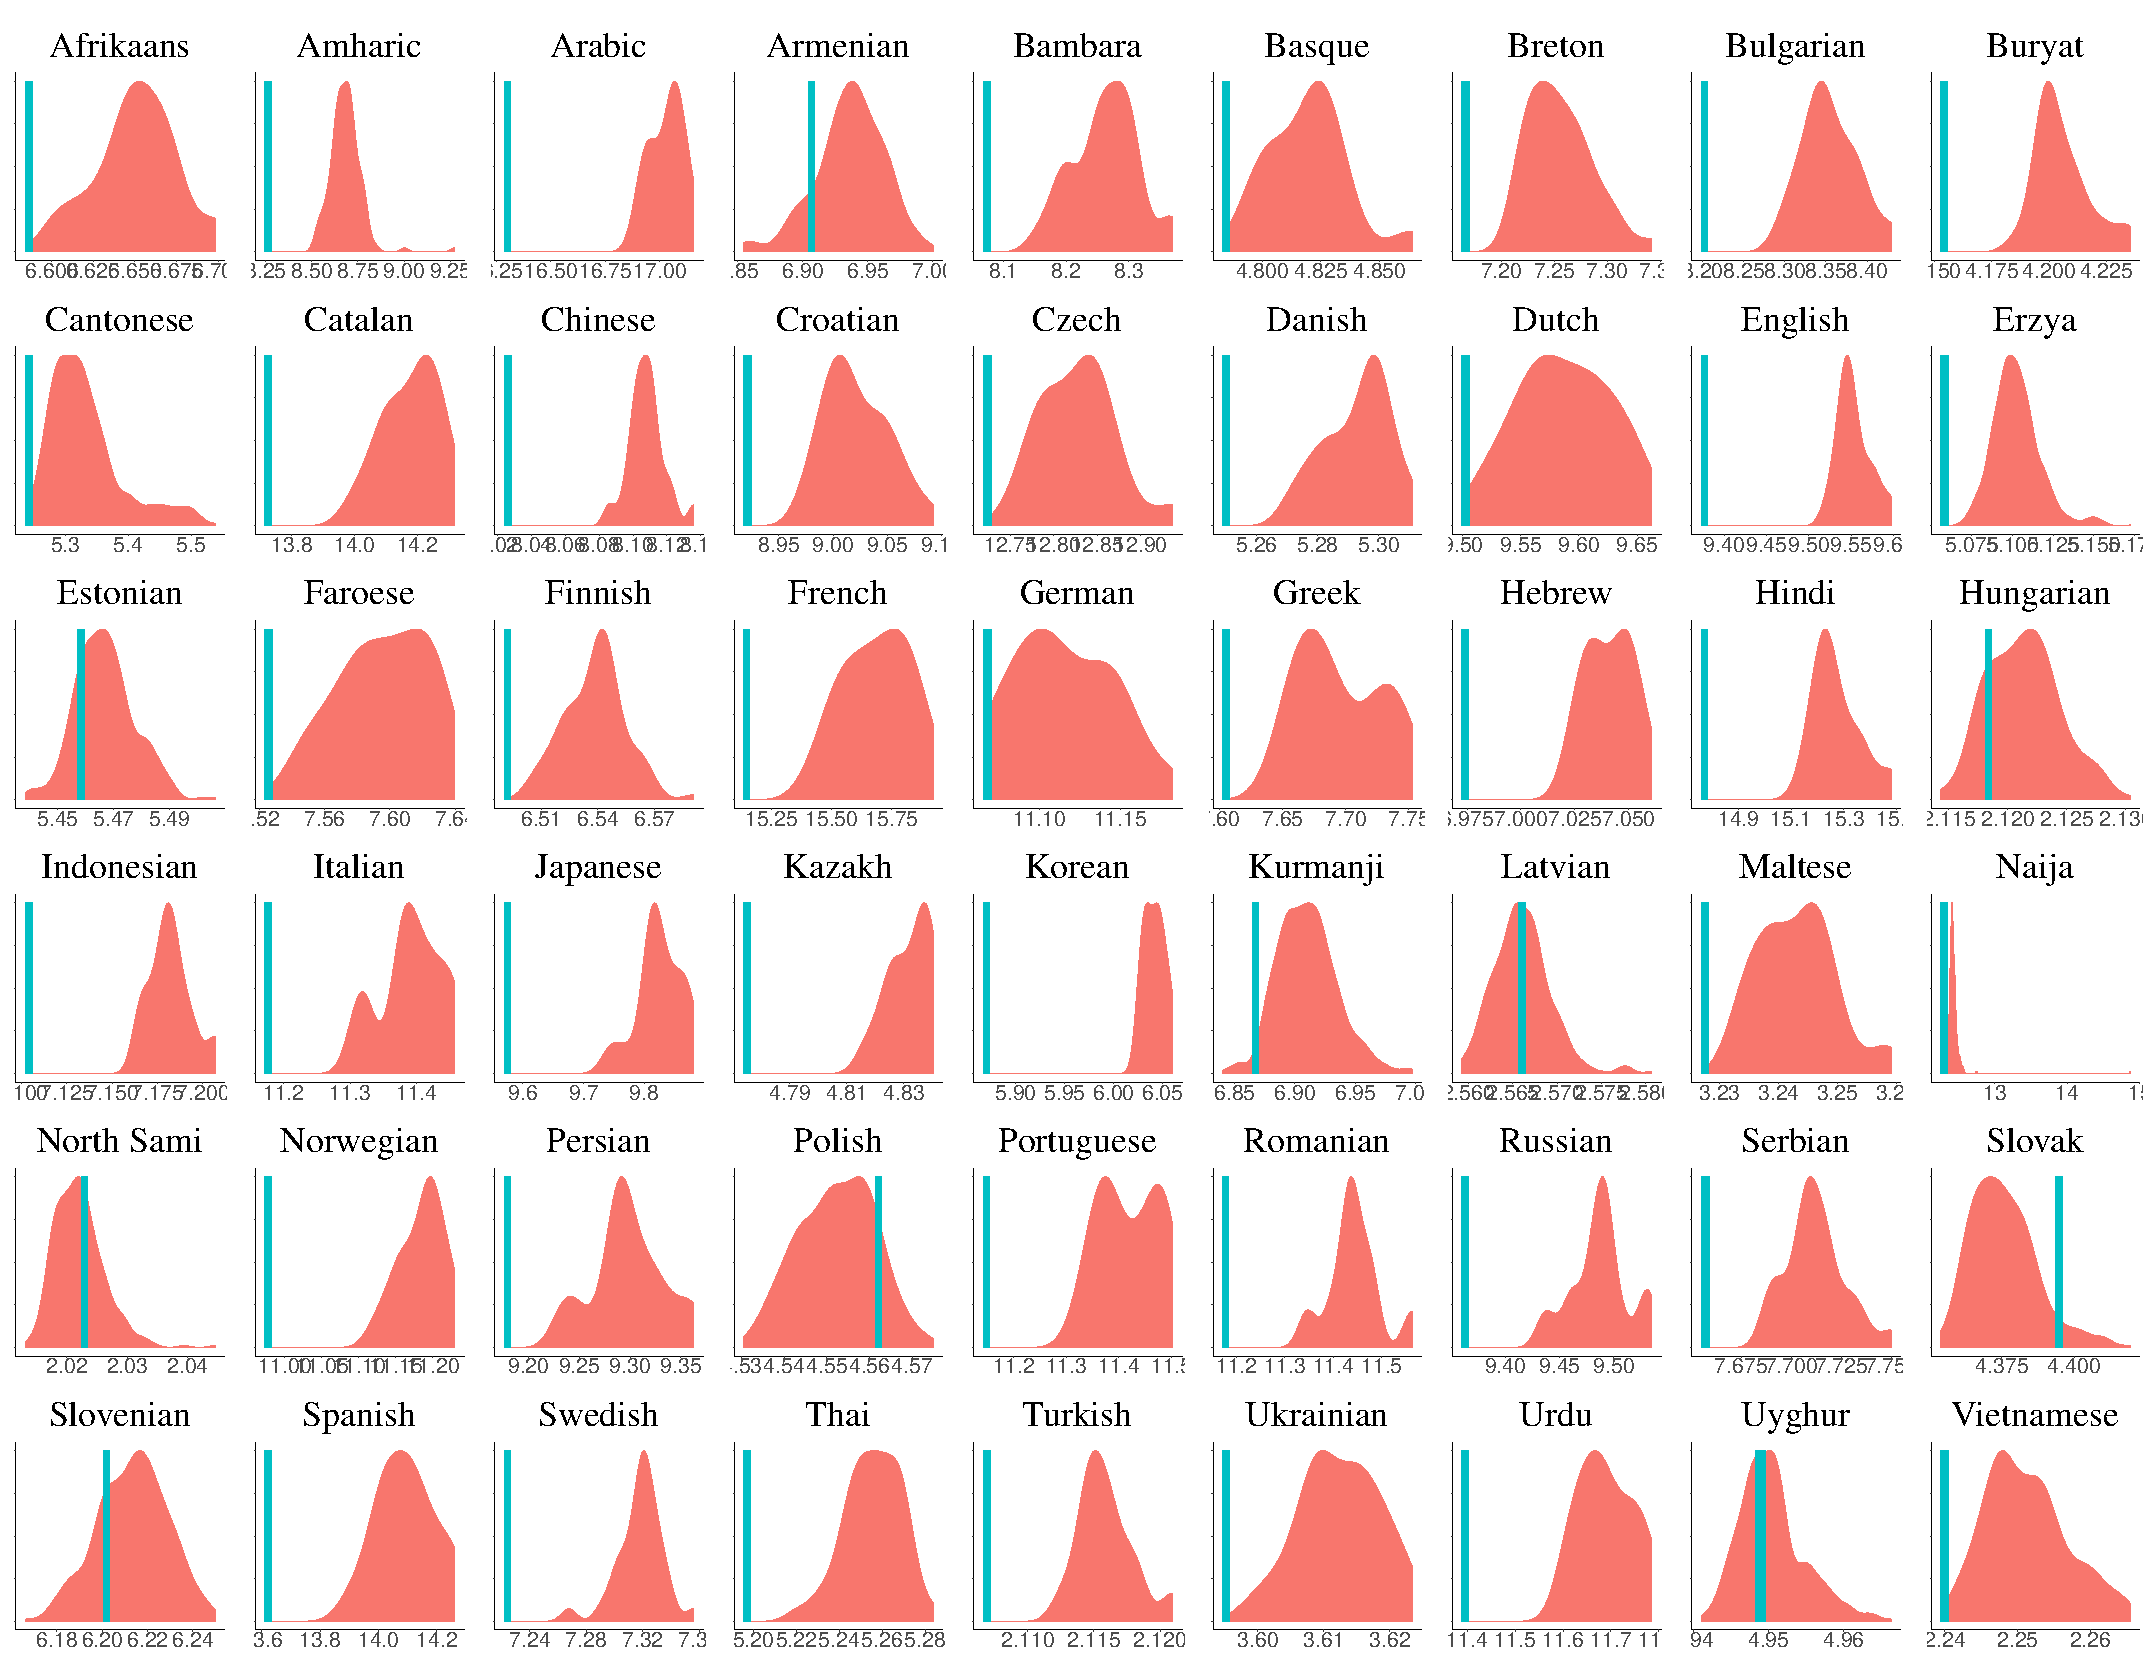
\includegraphics[width=\textwidth]{auc-table.pdf}
\end{center}
	\caption{AUC Histograms}\label{fig:auc}
\end{figure}



\begin{figure}
	\begin{center}
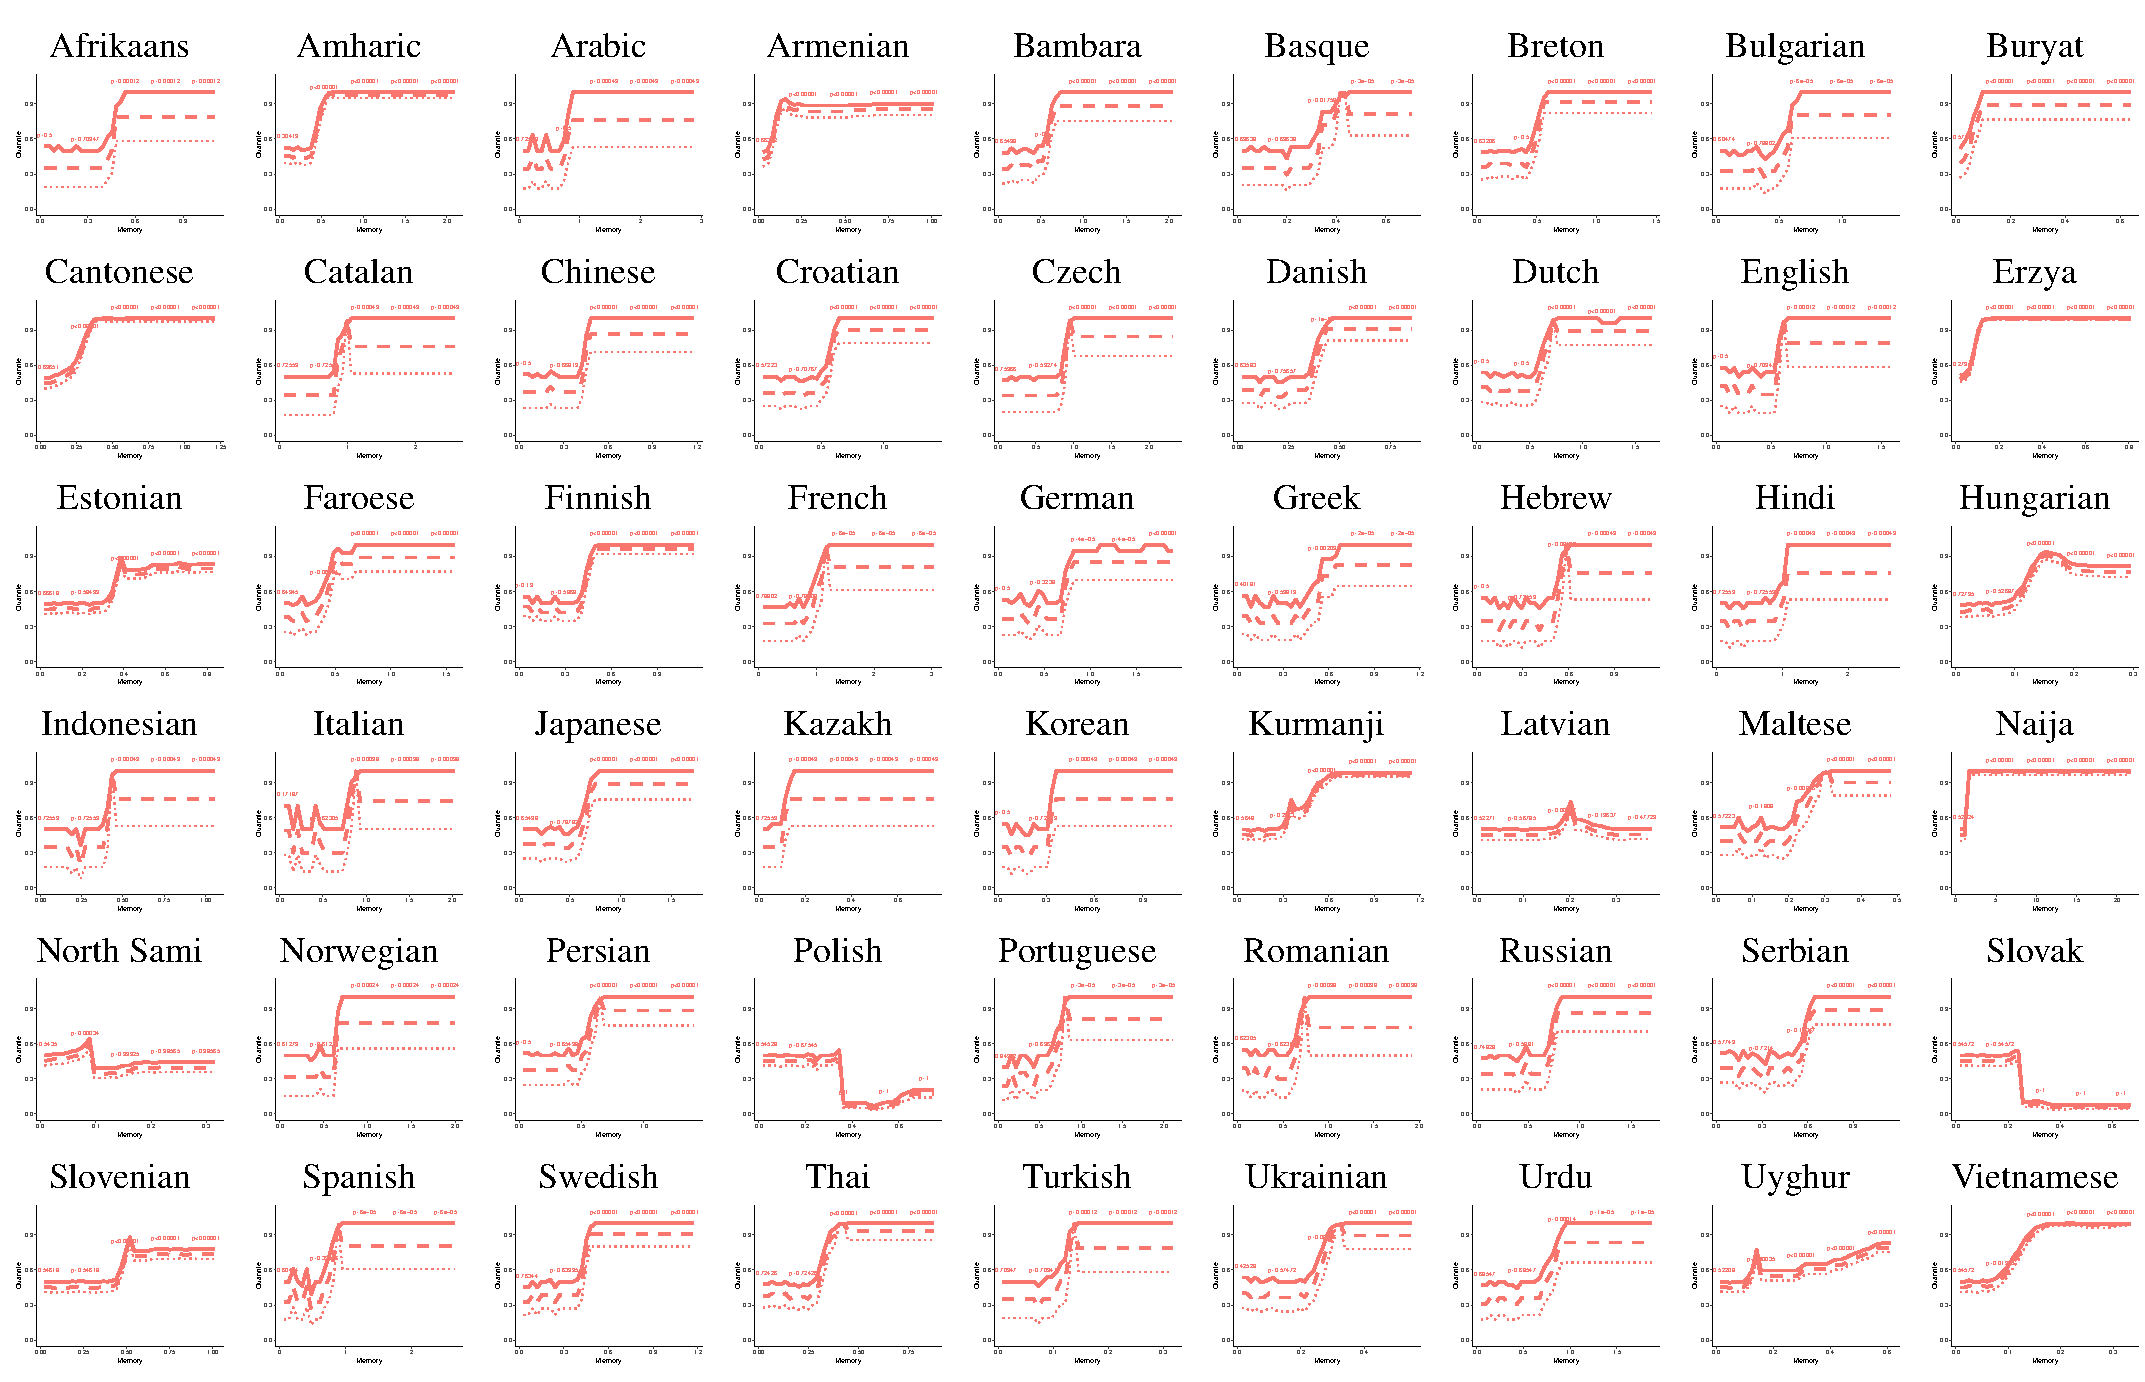
\includegraphics[width=\textwidth]{quantiles-table.pdf}
\end{center}
	\caption{Quantiles: At each given memory budget, what fraction of baseline grammars leads to higher surprisal?}\label{fig:quantile-table}
\end{figure}



%The numbers of samples taken per language are provided in SI Table~\ref{tab:samples}.

%In Figure~\ref{tab:plain-results} (TODO), we show the estimated memory-surprisal tradeoff curves for all samples.


In Figure~\ref{fig:it}, we show the estimated values of $I_t$ for all languages.
In most languages, $I_1$ is distinctly larger for the actual orderings (blue) compared to the baseline orderings (red). This means that real orderings tend to have 

In Figure~\ref{tab:medians}, we show the median surprisal at given levels of memory, for real and baseline languages.
We compute surprisal at 40 evenly spaced points of memory (selected individually for each language), over all runs for the real language, and over all baselines grammars.
We then compute the median surprisal over all runs for the real language, and over all baselines grammars.
For each point, we compute a confidence interval for the median surprisal, using the binomial PDF. \mhahn{some standard stats reference}
This is an \emph{exact} confidence interval, without parametric assumptions or asymptotic approximations.

Numerically, the real language provides better tradeoffs than the median of the baselines across languages, with four exceptions (Latvian, North Sami, Polish, Slovak).

In order to quantify the \emph{degree} of optimality, we compute what \emph{fraction} of baseline languages provides better tradeoffs than the real language.
At five evenly spaced memory values $\mu$ (chosen per language), we estimate what percentage $W_-(\mu)$ of baseline languages have lower (or equal) surprisal than the real language.
We use the Binomial Test to derive a confidence lower bound for this quantile (CITE), and to test against the null hypothesis that
\begin{equation}
	W_-(\mu) = 0.5
\end{equation}
In this test, we approximate the surprisal value of the real language by the \emph{sample median}.
Again, we take the real values to be estimated exactly by their medians.
Results are shown in Figure~\ref{fig:quantile-table}.

In all but the four exceptional languages, the real language had significantly lower surprisal than at least $50\%$ of the baseline languages for at least some values of $\mu$ at $p < 0.01$.
Also, for those languages, there was no $\mu$ where this pattern of significance was reversed.

We further computed the area under the memory-surprisal tradeoff curve (AUC) for real and baseline orderings.
In Figure~\ref{fig:auc}, we plot the AUC for the real orderings, together with the distribution of AUCs for baseline grammars.

%\subsection{Statistical Analysis}

%We now describe how we compared memory-surprisal tradeoffs between real and baseline languages.
%We want to test whether languages' surprisal-memory tradeoffs better than those of most baseline languages.
%We compare real and baseline languages by evaluating which languages result in lower surprisal at the same level of memory.
%We now describe the statistics we use to quantifying the difference between real and baseline languages.
%We do everything in a frequentist framework (null hypothesis testing \& confidence intervals), as we can do exact tests and confidence intervals without parametric assumptions.
%\mhahn{Maybe we can explain how the tests \& CIs also have reasonable Bayesian interpretations (for the specific methods used here, rejection of the null should guarantee that the posterior of the null hypothesis is small under a wide range of priors.).}

%\paragraph{Median Surprisal and Confidence Interval for Medians}



%\paragraph{CI for Median Difference}
%We create (nonparametric and nonasymptotic) confidence interval for the difference between real and baseline median surprisals at each memory value.
%\mhahn{the resulting plots are not very intuitive, might scrap this}
%
%% yStudyTradeoff_Bootstrap_Parallel_OnlyWordForms_BoundedVocab_BinomialTest_Single_MedianDiffCI.py



%This statistic also should have a reasonable Bayesian interpretation:
% E.g., if the random samples are unimodal, and we do inference over only the median (location family), 



%\begin{figure}
%	\begin{center}
%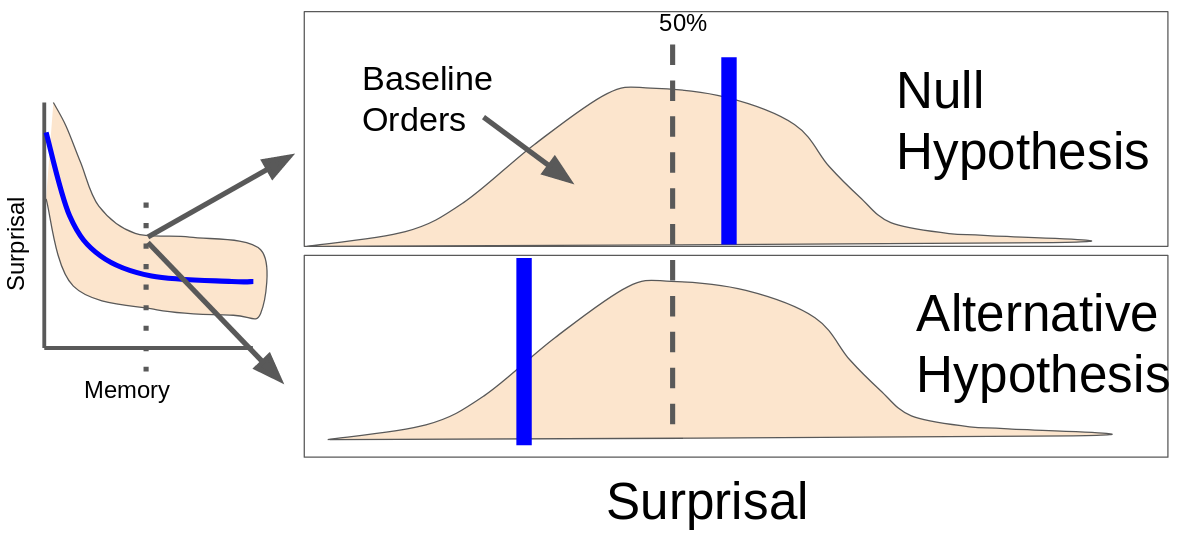
\includegraphics[width=0.45\textwidth]{figures/nhst.png}
%\end{center}
%	\caption{Illustration for the pointwise null-hypothesis significance test. At a given level of memory, we test against the null hypothesis that at least half of the baseline orders provide lower surprisal than the real language.}\label{fig:nhst-pointwise}
%\end{figure}






%For each memory value $\mu$, we do a significance test (nonparametric and nonasymptotic).
%\begin{equation}
%	W_+(\mu) \geq W_-(\mu)
%\end{equation}
%We use the empirical median for the real language.

% yStudyTradeoff_Bootstrap_Parallel_OnlyWordForms_BoundedVocab_BinomialTest_Single.py

%We take the REAL values to be estimated exactly by their medians.

%TODO some aggregate visualization of the quantiles
%\paragraph{AUC}
%TODO some aggregate visualization

%\begin{figure}
%	\begin{center}
%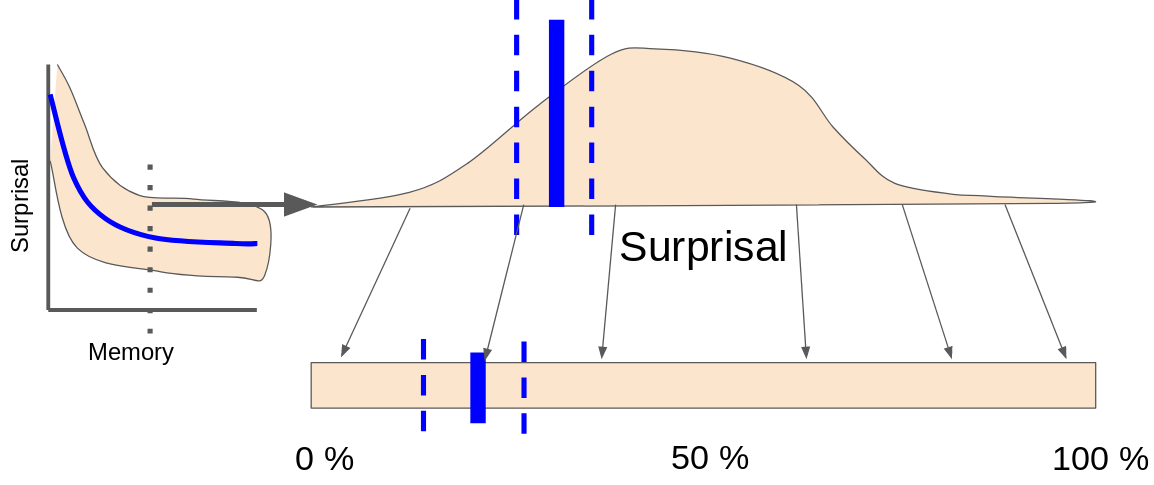
\includegraphics[width=0.45\textwidth]{figures/quantile.png}
%\end{center}
%	\caption{Illustration for the quantile estimate. At each level of memory, we provide an estimate of the percentage of baseline languages that have lower surprisal than the real language.}\label{fig:quantile-pointwise}
%\end{figure}



%Also the following does not assume unimodality, and ends up getting about the same intervals
%% yStudyTradeoff_Bootstrap_Parallel_OnlyWordForms_BoundedVocab_BinomialTest_Single_UnimodalBoundOnQuantile_BothDirections_NoAssumption.py






%In Figure~\ref{tab:slice-hists-real}, we show the distribution of surprisals achieved at the maximal memory value for real and random languages.

%In Figure~\ref{fig:hist-real}, we show surprisals at maximum memory, after z-transforming for each individual language and then aggregating.

%In Table \ref{tab:median_diffs}, we show the differences in median surprisal, as a function of memory.


%In Table~\ref{tab:boot-g}, we report the bootstrap estimates and confidence intervals for G~(\ref{eq:g}).
%$\E[G]$ was not estimated to be significantly above $>5$ for four languages: Latvian, North Sami, Polish, and Slovak.


%In Table~\ref{tab:quantiles}, we show the quantiles.





\subsection{Discussion}

We have found that 50 out of 54 languages provide better memory-surprisal tradeoffs than random baselines with consistent but counterfactual word order rules.

Four languages provide exceptions; these are Latvian (Baltic), North Sami (Uralic), Polish and Slovak (both Slavic).
All four languages have strong word order freedom (CITE).
Freedom of word order plausibly makes sentences less predictable, as the same syntactic structure can receive different surface realizations.
We thus hypothesized that freedom of word order impacts the memory-surprisal tradeoff, and that languages with more strongly fixed word order should display more optimal memory-surprisal tradeoffs.

To test this hypothesis, we examined the correlation between word order freedom and the surprisal difference between real and baseline orderings.
To quantify word order freedom, we used a corpus-based estimate, the \emph{branching direction entropy}~\citep{futrell-quantifying-2015}.
This is the entropy of the ordering (head-first or dependent-first) of dependencies conditioned on the dependency label and the part-of-speech label of head and dependent.
These two quantities are plotted in Figure~\ref{fig:hist-real}.
We found that branching direction entropy was strongly correlated with the surprisal difference between real and baseline orderings (Spearman correlations -0.58, $p = 7.414e-6$).

We will address this in Experiment 3.


\begin{figure}
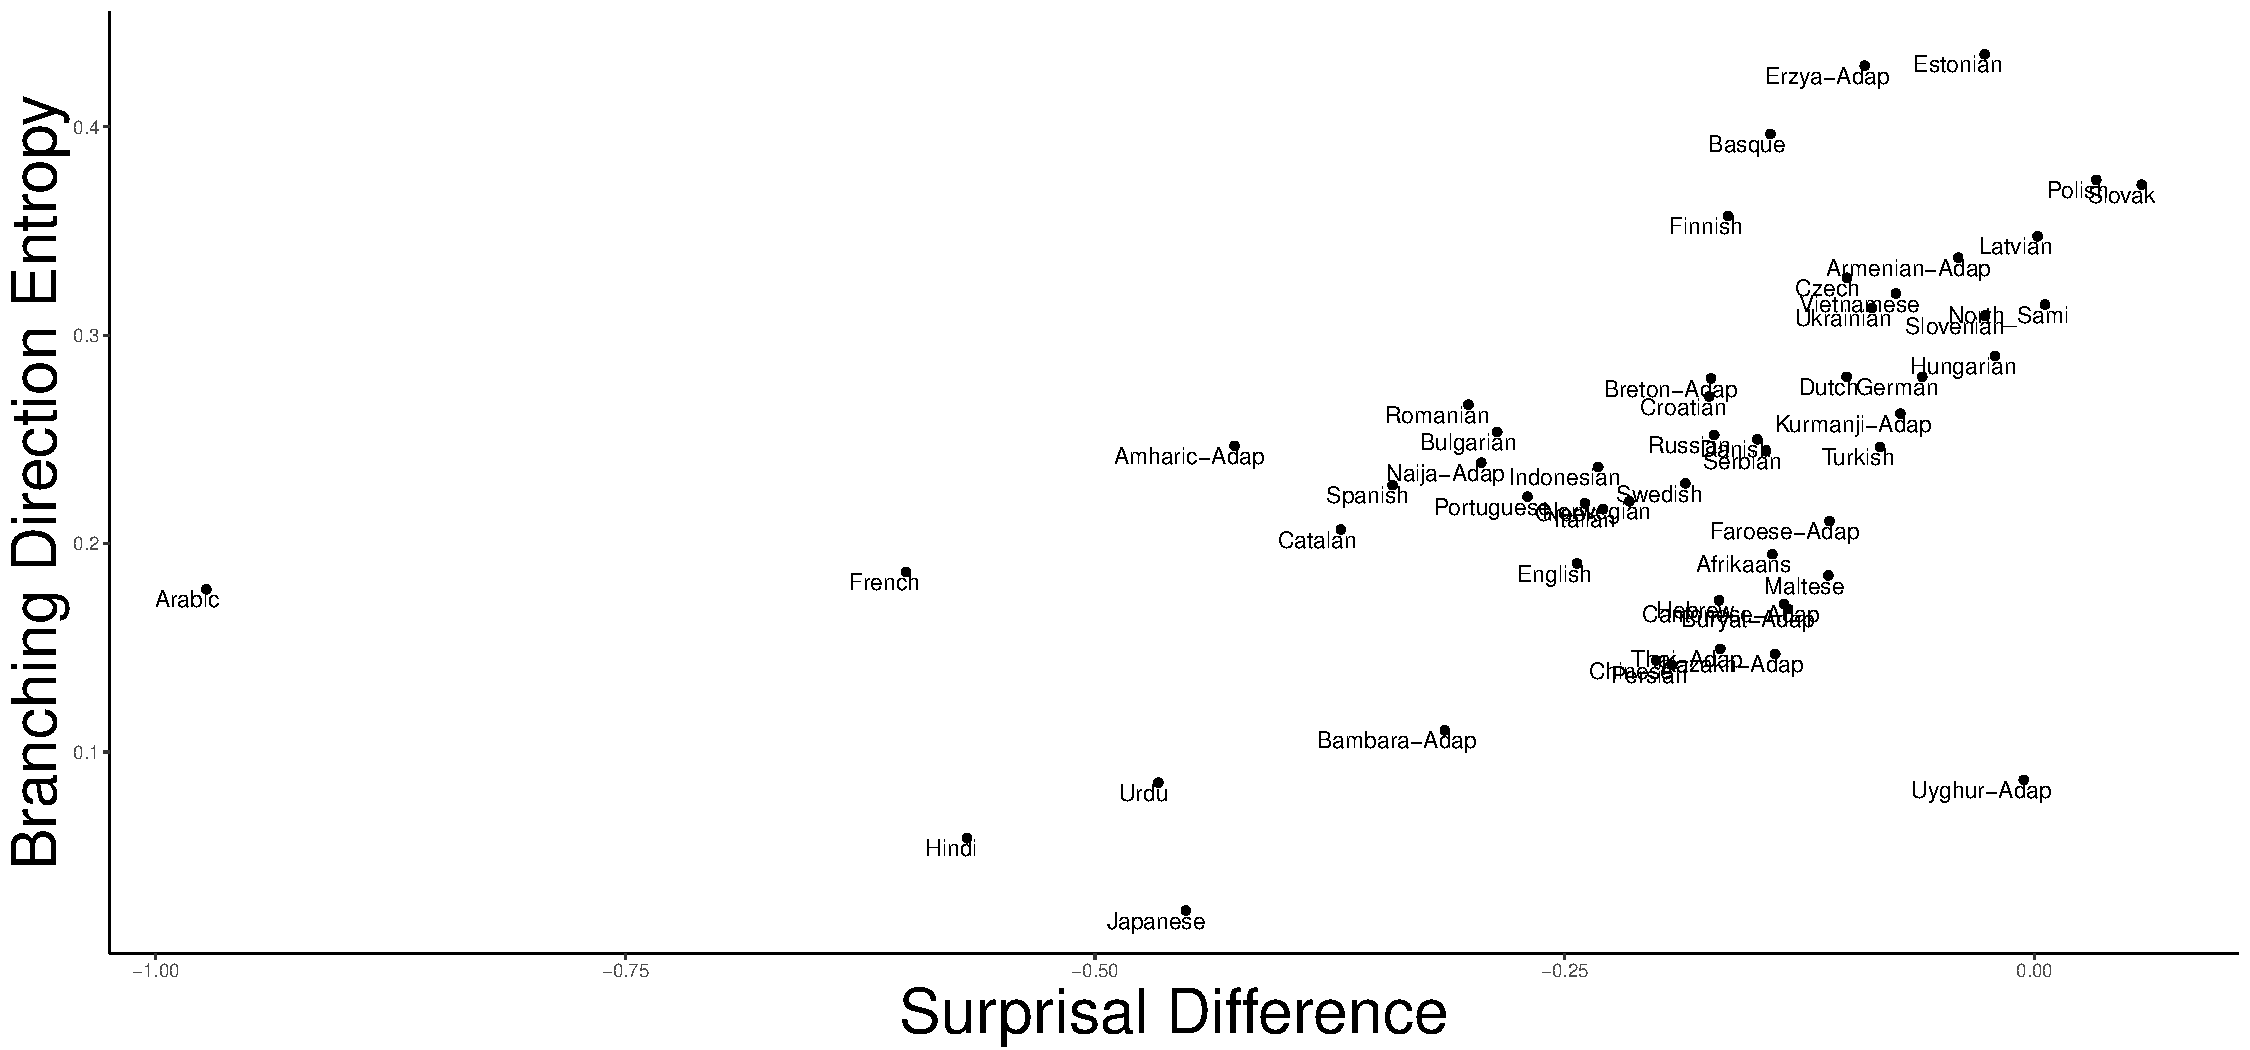
\includegraphics[width=0.95\textwidth]{figures/surprisal-branching-entropy-REAL.pdf}
	\caption{Surprisal Difference vs Branching Direction Entropy.}\label{fig:hist-real}
\end{figure}


\mhahn{One thing that has to be discussed: the absolute values differ between languages}



A possible concern is that the optimization observed in Experiment 1 might be an artifact of the grammar formalism.
We will address this in Experiment 3.
%To address this possibility, we repeated the experiment comparing baseline grammars to grammars that represent the word order of the real languages as faithfully as is possible with the grammar formalism.


